\documentclass[25pt,a0paper,portrait,dvipsnames,innermargin=0.4in,colspace=0.4in,blockverticalspace=0.4in]{tikzposter}

\tikzposterlatexaffectionproofoff

\usepackage{amssymb}
\usepackage{libertine}
\usepackage{listings}
\usepackage[most]{tcolorbox}

\definecolor{ProfessionalGreen}{RGB}{0, 104, 106}
\definecolor{ProfessionalDarkGreen}{RGB}{0, 33, 34}

\definecolorstyle{MyPoster}{
  \definecolor{colorOne}{named}{ProfessionalGreen}
  \definecolor{colorTwo}{named}{RedOrange}
  \definecolor{colorThree}{named}{RoyalBlue}
}{
  % Background Colors
  \colorlet{backgroundcolor}{white}
  \colorlet{framecolor}{black}
  % Title Colors
  \colorlet{titlefgcolor}{colorOne!5!white}
  \colorlet{titlebgcolor}{colorOne}
  % Block Colors
  \colorlet{blocktitlebgcolor}{ProfessionalDarkGreen}
  \colorlet{blocktitlefgcolor}{ProfessionalDarkGreen!10!white}
  \colorlet{blockbodybgcolor}{ProfessionalDarkGreen}
  \colorlet{blockbodyfgcolor}{ProfessionalDarkGreen!10!white}
  % Innerblock Colors
  \colorlet{innerblocktitlebgcolor}{white}
  \colorlet{innerblocktitlefgcolor}{black}
  \colorlet{innerblockbodybgcolor}{colorThree!30!white}
  \colorlet{innerblockbodyfgcolor}{black}
  % Note colors
  \colorlet{notefgcolor}{black}
  \colorlet{notebgcolor}{colorTwo!50!white}
  \colorlet{noteframecolor}{colorTwo}
}
\settitle{\vbox{
  \hspace*{2in}
  \colorbox{white}{\hbox to 4in {\vbox to 4.4in {\vspace*{1.8in} \raisebox{-0.5\height}{\@titlegraphic}}}}
  \hspace*{-6.8in}
  \vbox{
    % \@titlegraphic\\[\TP@titlegraphictotitledistance]
    \raggedleft
    \vspace*{0.8in}
    \color{titlefgcolor} {\bfseries \Huge \sc \@title \hspace*{0.5in} \par}
    \vspace*{0.8in}
    \vbox{
      {\LARGE \@author \par} \vspace*{0.1in} {\large https://Ailrun.github.io \par} \vspace*{0.3in} {\large \@institute \par}
      \vspace*{0.1in} {\large https://complogic.cs.mcgill.ca/}
    }
    \vspace*{-0.2in}
  }
}}

\defineblockstyle{MyBlock}{
  titlewidthscale=1, bodywidthscale=1, titleleft,
  titleoffsetx=0in, titleoffsety=0in, bodyoffsetx=0in, bodyoffsety=0.6in,
  bodyverticalshift=0.6in, roundedcorners=2, linewidth=5pt,
  titleinnersep=0.3in, bodyinnersep=0.3in
}{
  \begin{scope}[line width=\blocklinewidth, rounded corners=\blockroundedcorners]
    \ifBlockHasTitle %
      \draw[color=blocktitlebgcolor, fill=blocktitlebgcolor] (blockbody.south west) rectangle (blocktitle.north east);
      \draw[color=blocktitlebgcolor, fill=blockbodybgcolor] (blockbody.south west) rectangle (blockbody.north east);
      \draw[color=blocktitlefgcolor, thin] ($(blocktitle.south west) + (1em,0)$) -- ($(blocktitle.south east) + (-1em, 0)$);
    \else
      \draw[color=blocktitlebgcolor, fill=blockbodybgcolor] (blockbody.south west) rectangle (blockbody.north east);
    \fi
  \end{scope}
}

% \usetheme{Autumn}
\usetitlestyle[titletoblockverticalspace=0.5in,innersep=0in,linewidth=0in]{Filled}
\usecolorstyle{MyPoster}
\useblockstyle[roundedcorners=2]{MyBlock}

\newenvironment{tikzfigure*}[1][]{
  \def \rememberparameter{#1}
  \vspace{10pt}
  \begin{center}
  }{
    \ifx\rememberparameter\@empty
    \else %nothing
    {\small \rememberparameter}
    \fi
  \end{center}
}

\lstdefinelanguage{Moebius}%
{%
  keywords=%
  {%
    box,with,%
    Fun,fun,%
    if,else,then,match,%
    let,in,%
    case,of,%
    type,%
  },%
  sensitive,
  morecomment=[l]{--},%
  moredelim=[is][\color{orange}]{o<<}{>>o},%
  moredelim=[is][\color{violet}]{v<<}{>>v},%
  moredelim=[is][\color{ForestGreen}]{fg<<}{>>fg},%
  moredelim=[is][\color{NavyBlue}]{nb<<}{>>nb},%
  moredelim=[is][\color{WildStrawberry}]{ws<<}{>>ws},%
  moredelim=[is][\color{white}]{w<<}{>>w},%
  moredelim=[is][\underline]{u<<}{>>u},%
}
% \lstset{%
%   basicstyle=\ttfamily\footnotesize,%
%   keywordstyle=\color{blue}\bfseries,%
%   numberstyle=\ttfamily\bfseries\color{gray}\footnotesize,%
%   literate=%
%   {->}{{\(\rightarrow\ \)}}2 %
%   {|-}{{\(\vdash\)}}2 %
%   {\\alpha}{{\(\alpha\)}}1 %
%   {\\beta}{{\(\beta\)}}1 %
%   {\\tau}{{\(\tau\)}}1 %
%   {\\sigma}{{\(\sigma\)}}1 %
%   {\\rho}{{\(\rho\)}}1 %
%   {\\Gamma}{{\(\Gamma\)}}1 %
%   {\\Psi}{{\(\Psi\)}}1 %
%   {[}{{\(\lceil\)}}1 % box
%   {]}{{\(\rceil\)}}1 % box
%   {u<}{{\(\lfloor\)}}1 % unbox
%   {>u}{{\(\rfloor\)}}1 % unbox
%   {v[}{[}1 % list
%   {]v}{]}1 % list
%   ,%
%   mathescape=true,%
%   xleftmargin=0.05in,%
%   resetmargins=true,%
%   belowskip=0.05in,%
%   aboveskip=0.05in,%
% }
\lstset{
  basicstyle=\small\color{black!5!white}\ttfamily,%
  keywordstyle=\color{orange},%
  xleftmargin=0.8in,%
  xrightmargin=0.8in,%
  belowskip=0in,%
  framextopmargin=0.2in,%
  framexbottommargin=0.2in,%
  framexleftmargin=0.2in,%
  framexrightmargin=0.2in,%
  framesep=0in,%
  frame=single,%
  framerule=0in,%
  backgroundcolor=\color{black},%
  mathescape=true,
  literate=%
  {_1}{{\(_1\)}}1 %
  {_2}{{\(_2\)}}1 %
  {^n}{{\(^n\)}}1 %
  {^0}{{\(^0\)}}1 %
  {^1}{{\(^1\)}}1 %
  {^2}{{\(^2\)}}1 %
  {^3}{{\(^3\)}}1 %
  {Box}{{\(\Box\)}}1 %
  {Gamma}{{\(\Gamma\)}}1
  {sigma}{{\(\sigma\)}}1
  {|-}{{\(\vdash\)}}1
  {->}{{\(\rightarrow\)}}1
  ,%
}
\lstloadlanguages{Moebius}
\lstset{language=Moebius}

\tcbset{
  on line,%
  boxsep=0.2em,%
  left=0pt,%
  right=0pt,%
  top=0pt,%
  bottom=0pt,%
  colframe=black,%
  colback=black,%
  highlight math style={enhanced},%
}

\newcommand\moeb[1]{\tcbox{\lstinline[flexiblecolumns=false]{#1}}}

\begin{filecontents*}[overwrite]{src/untyped-nth.premoebius}
ws<<untypedNth>>ws n = if n <= 0 then box(nb<<head xs>>nb)
                         else let box(C) = ws<<untypedNth>>ws (n - 1) in
                              box(nb<<let xs = tail xs in>>nb C)
\end{filecontents*}

\begin{filecontents*}[overwrite]{src/untyped-nth-2-result.premoebius}
box(nb<<let xs = tail xs in
    let xs = tail xs in
    head xs>>nb)
\end{filecontents*}

\begin{filecontents*}[overwrite]{src/int-nth.moebius}
ws<<intNth>>ws : fg<<Int -> Box (Int list -> Int)>>fg
ws<<intNth>>ws n = if n <= 0 then box(nb<<fun xs => head Int xs>>nb)
                     else let box(C) = ws<<intNth>>ws (n - 1) in
                          box(nb<<fun xs =>>>nb C nb<<(tail Int xs)>>nb)
\end{filecontents*}

\begin{filecontents*}[overwrite]{src/int-nth-2-result.moebius}
box(nb<<fun xs =>
      (fun xs =>
        (fun xs => head xs)
        (tail xs))
      (tail xs)>>nb)
\end{filecontents*}

\begin{filecontents*}[overwrite]{src/polymorphic-nth-wrong.moebius}
ws<<badPolyNth>>ws : fg<<('a : Type) -> Int -> Box ('a list -> 'a)>>fg
ws<<badPolyNth>>ws 'a n = if n <= 0 then box(nb<<fun xs => head 'a xs>>nb)
                            else let box(C) = ws<<badPolyNth>>ws 'a (n - 1) in
                                 box(nb<<fun xs =>>>nb C nb<<(tail 'a xs)>>nb)
\end{filecontents*}

\begin{filecontents*}[overwrite]{src/matching.moebius}
ws<<nthToOneBefore>>ws : fg<<Box (Int list -> Int) -> Box (Int list -> Int)>>fg
ws<<nthToOneBefore>>ws nthCode = case nthCode of
  | box(nb<<fun xs => head xs>>nb)     -> box(nb<<fun xs => head xs>>nb)
  | box(nb<<fun xs =>>>nb u<<X>>u nb<<(tail xs)>>nb) -> box(u<<X>>u)
\end{filecontents*}

\begin{filecontents*}[overwrite]{src/open-int-nth.moebius}
ws<<openIntNth>>ws : fg<<Int -> [xs : Int list |- Int]>>fg
ws<<openIntNth>>ws n = if n <= 0 then
                 box(nb<<xs>>nb . nb<<head Int xs>>nb)
               else
                 let box(nb<<xs>>nb . C) = ws<<openIntNth>>ws (n - 1) in
                 box(nb<<xs>>nb . C with nb<<(tail Int xs)>>nb)
\end{filecontents*}

\begin{filecontents*}[overwrite]{src/open-int-nth-2-result.moebius}
box(nb<<xs>>nb . nb<<head (tail (tail xs))>>nb)
\end{filecontents*}

\begin{filecontents*}[overwrite]{src/polymorphic-nth.moebius}
ws<<polyNth>>ws : fg<<('a : (|-^2 Type)) -> Int -> [xs : 'a list |-^1 'a]>>fg
ws<<polyNth>>ws 'a n = if n <= 0 then
                 box(nb<<xs>>nb .^1 nb<<head 'a xs>>nb)
               else
                 let box(xs .^1 C) = ws<<polyNth>>ws 'a (n - 1) in
                 box(nb<<xs>>nb .^1 C nb<<(tail 'a xs)>>nb)
\end{filecontents*}

\begin{filecontents*}[overwrite]{src/contextual-matching.moebius}
ws<<nthToOneBefore>>ws : ('a : (|-^2 Type)) -> fg<<[xs : 'a list |-^1 'a] -> [xs : 'a list |-^1 'a]>>fg
ws<<nthToOneBefore>>ws nthCode = case nthCode of
  | box(nb<<xs>>nb .^1 nb<<head xs>>nb) -> box(nb<<xs>>nb .^1 nb<<head xs>>nb)
  | box(nb<<xs>>nb .^1 nb<<head (tail>>nb u<<X>>unb<<)>>nb) -> box(nb<<xs>>nb .^1 nb<<head>>nb u<<X>>u)
\end{filecontents*}

\begin{document}
\title{Type System for Metaprogramming}
\author{Junyoung ``Clare'' Jang}
\date{\today}
\institute{Complogic Group}
\titlegraphic{
\includegraphics[width=4in]{./mcgill_sig_red.png}}
%% Abstract:
%% Metaprogramming is the art of generating, manipulating, and analyzing code. This technique is nearly universal: compilers, user libraries, and program analyzers use this technique for both better performance and easier maintenance. However, metaprogramming has been suffered from one issue: it is harder to write a reliable and safe metaprogram, especially because they are harder to test thoroughly. This poster will present how to give static reliability and safety guarantees using a type system on metaprograms, illustrated with issues in a type system for metaprogramming and our solutions.
\maketitle{}

\begin{columns}
  \column{0.5}
  \block{Metaprogramming}{
    \begin{tikzfigure*}
      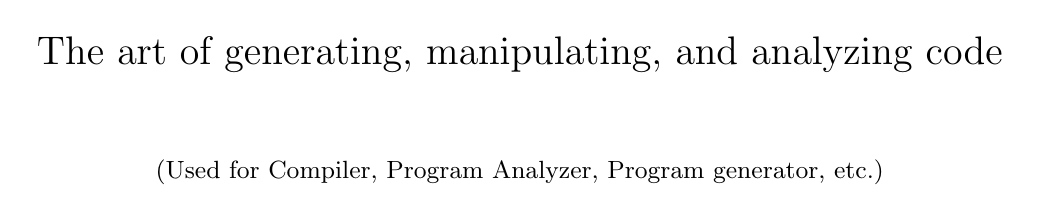
\begin{tikzpicture}
        \node at (0,1.5) {\Large The art of generating, manipulating, and analyzing code};
        \node at (0,0) {\small (Used for Compiler, Program Analyzer, Program generator, etc.)};
      \end{tikzpicture}
    \end{tikzfigure*}
    \begin{tikzfigure*}
      \usetikzlibrary{arrows}
      \pgfdeclarelayer{background}
      \pgfsetlayers{background,main,notelayer}
      % \small
      \begin{tikzpicture}
        \node[draw,text width=2.6in,align=center] (n0) at (10,0) {Program};
        \node[draw,text width=2.6in,align=center] (n4) at (28,0) {Result};
        \node[align=center] (nt) at (0,0) {\bfseries Direct Programming};

        \draw[-latex,line width=0.05in] (n0.east) -- (n4.west);

        \node[draw,text width=2.6in,align=center] (m0) at (10,-4) {Meta\--program};
        \node[draw,text width=2.7in,align=center] (m2) at (19,-4) {Object program};
        \node[draw,text width=2.6in,align=center] (m4) at (28,-4) {Result};
        \node[align=center] (mt) at (0,-4) {\bfseries Metaprogramming};

        \draw[-latex,line width=0.05in] (m0.east) -- (m2.west);
        \draw[-latex,line width=0.05in] (m2.east) -- (m4.west);

        \begin{pgfonlayer}{background}
          \filldraw[line width=0.5in,join=round,draw=colorOne,fill=colorOne]
          (n0.north  -| n0.west) rectangle (n4.south  -| n4.east)
          (m0.north  -| m0.west) rectangle (m4.south  -| m4.east);
        \end{pgfonlayer}
      \end{tikzpicture}
    \end{tikzfigure*}
  }
  \block{Metaprogramming with Box/Let-box}{
    \begin{tikzfigure*}
      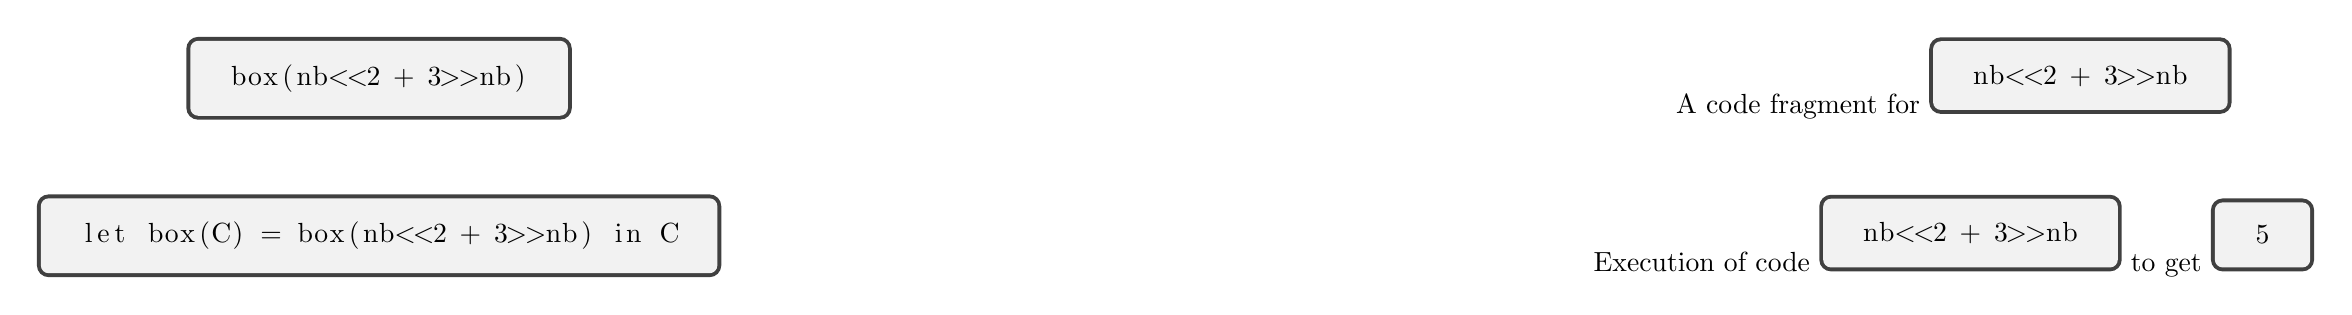
\begin{tikzpicture}
        \draw (0,2) node {\moeb{box(nb<<2 + 3>>nb)}} (20,2) node {A code fragment for \moeb{nb<<2 + 3>>nb}};
        \draw (0,0) node {\moeb{let box(C) = box(nb<<2 + 3>>nb) in C}} (20,0) node {Execution of code \moeb{nb<<2 + 3>>nb} to get \moeb{5}};
      \end{tikzpicture}
    \end{tikzfigure*}
    \begin{tikzfigure*}[Untyped metaprogram to get the \(n\)-th item in a list]
      \lstinputlisting{src/untyped-nth.premoebius}
    \end{tikzfigure*}
    If we evaluate \moeb{ws<<untypedNth>>ws 2}, we get
    \begin{tikzfigure*}
      \lstinputlisting{src/untyped-nth-2-result.premoebius}
      % \usetikzlibrary{arrows.meta}
      % \pgfdeclarelayer{background}
      % \pgfsetlayers{background,main,notelayer}
      % \begin{tikzpicture}
      %   % double=blocktitlebgcolor,double distance=0.05in,
      %   \node (a) at (18,0) {\moeb{box(nb<<let xs = tail xs in head xs>>nb)}};
      %   \draw[line width=0.02in,double=blocktitlebgcolor,double distance=0.05in,-Implies] (b.east) -- (a.west);
      % \end{tikzpicture}
    \end{tikzfigure*}}

  \block{\emph{Typed} Metaprogramming}{
    What if
    \begin{itemize}
    \item There is no variable \(xs\) when executing the code from \moeb{ws<<untypedNth>>ws 2}?
    \item The variable \(xs\) is not a list when executing the code from \moeb{ws<<untypedNth>>ws 2}?\\
    \end{itemize}

    We want to ensure that generated code will be well-typed \emph{before} executing a meta-program.
    \begin{tikzfigure*}
      \usetikzlibrary{arrows}
      \pgfdeclarelayer{background}
      \pgfsetlayers{background,main,notelayer}
      \begin{tikzpicture}
        \node[draw,orange,text width=2.6in,align=center] (mts) at (10,0) {Type System};
        \node[draw,orange,text width=2.6in,align=center] (m0) at (10,-4) {Meta\--program};
        \node[draw,red!30!white,text width=2.7in,align=center] (m2) at (19,-4) {Object program};
        \node[draw,text width=2.6in,align=center] (m4) at (28,-4) {Result};
        % \node[align=center] (mt) at (0,-4) {\bfseries Metaprogramming};

        \draw[-latex,line width=0.05in] (m0.east) -- (m2.west);
        \draw[-latex,line width=0.05in] (m2.east) -- (m4.west);

        \draw[orange,-latex,line width=0.05in] (mts.south) -- node[pos=0.5,anchor=east] (mtc) {Type Check} (m0.north);
        \draw[red!30!white,-latex,line width=0.05in] (mts.east) -| node[pos=0.5,anchor=west] (mgt) {Guarantee Well-Typedness} (m2.north);

        \begin{pgfonlayer}{background}
          \filldraw[line width=0.5in,join=round,draw=colorOne,fill=colorOne]
          (mts.north  -| mtc.west) rectangle (m4.south  -| m4.east);
        \end{pgfonlayer}
      \end{tikzpicture}
    \end{tikzfigure*}}

  % Judgment - explanation form
  % Rule - explanation form
  % Connection between ``necessity'' and ``code fragment''
  \block{Modal Logic}{
    \begin{tikzfigure*}
      \usetikzlibrary{arrows.meta}
      \pgfdeclarelayer{background}
      \pgfsetlayers{background,main,notelayer}
      \begin{tikzpicture}
        \node[draw,text width=4.5in,align=center] (codel) at (0, 0) {Well-typed Closed Code Fragment};
        \node[draw,text width=4.5in,align=center] (coder) at (18, 0) {Well-typed under\\{}\emph{Any} Environment};

        \draw[Implies-Implies,line width=0.02in,double=colorOne,double distance=0.05in,shorten <=0.1in,shorten >=0.1in] (codel) -- (coder);

        \node[draw,text width=4.5in,align=center] (modall) at (0, -4) {Necessary Truth (in S4)};
        \node[draw,text width=4.5in,align=center] (modalr) at (18, -4) {True under \emph{Any} World};

        \draw[Implies-Implies,line width=0.02in,double=colorOne,double distance=0.05in,shorten <=0.1in,shorten >=0.1in] (modall) -- (modalr);

        \begin{pgfonlayer}{background}
          \filldraw[line width=0.5in,join=round,draw=colorOne,fill=colorOne]
          (codel.north  -| codel.west) rectangle (modalr.south  -| modalr.east);
        \end{pgfonlayer}
      \end{tikzpicture}
    \end{tikzfigure*}
    \begin{tikzfigure*}
      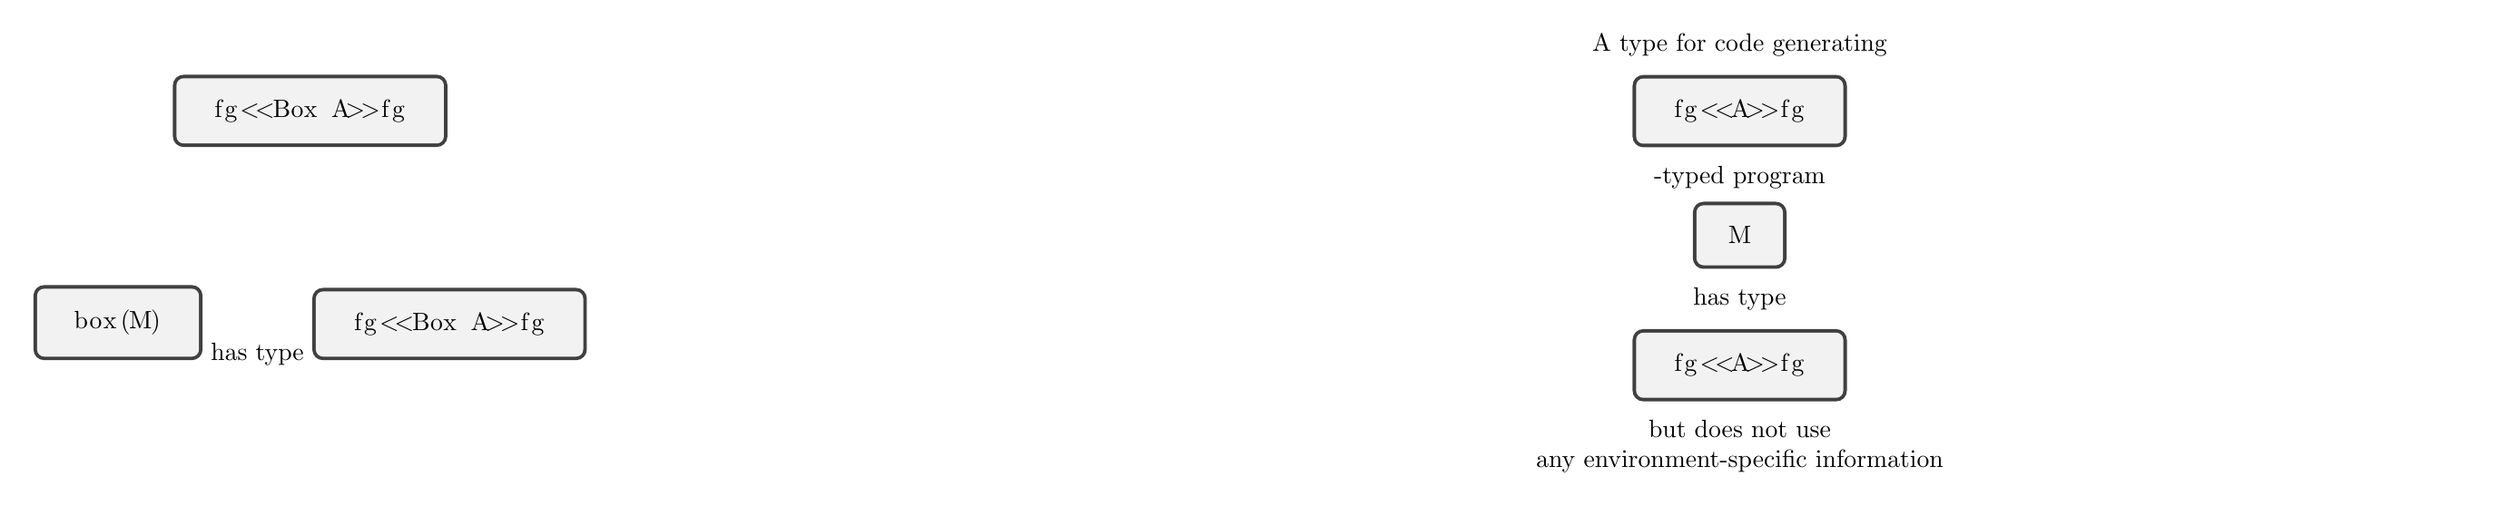
\begin{tikzpicture}
        \draw (0,3) node {\moeb{fg<<Box A>>fg}} (20,3) node[text width=8in,align=center] {A type for code generating \moeb{fg<<A>>fg}-typed program};
        \draw (0,0) node {\moeb{box(M)} has type \moeb{fg<<Box A>>fg}} (20,0) node[text width=8in,align=center] {\moeb{M} has type \moeb{fg<<A>>fg} but does not use\\ any environment-specific information};
      \end{tikzpicture}
    \end{tikzfigure*}
    \begin{tikzfigure*}[Typed metaprogram to get the \(n\)-th item in an int list]
      \lstinputlisting{src/int-nth.moebius}
    \end{tikzfigure*}
    If we execute \moeb{ws<<intNth>>ws 2}, we get
    \begin{tikzfigure*}
      \lstinputlisting{src/int-nth-2-result.moebius}
    \end{tikzfigure*}}

  \block{Problem 1 \---- Well-typed Open Code Fragments}{\moeb{ws<<untypedNth>>ws 2} has a free variable \moeb{xs}, but we cannot type check this as-is with Simple S4. Thus, \moeb{ws<<intNth>>ws 2} has some redundant anonymous functions and function calls.}

  \column{0.5}
  \block{Problem 2 \---- Polymorphism}{\moeb{ws<<intNth>>ws 2} works only for \moeb{ws<<Int>>ws} lists. The following approach to polymorphism does not work:
    \begin{tikzfigure*}[Ill-typed polymorphic metaprogram to get the \(n\)-th item in a list]
      \lstinputlisting{src/polymorphic-nth-wrong.moebius}
    \end{tikzfigure*}
    because code \moeb{nb<<fun xs => head 'a xs>>nb} depends on \moeb{'a} and thus is not closed.}

  \block{Problem 3 \---- Pattern Matching on Code Fragments}{
    \begin{tikzfigure*}[Metaprogram analyzing a code fragment from \moeb{nth} to get code for the \((n-1)\)-th item]
      \lstinputlisting{src/matching.moebius}
    \end{tikzfigure*}
    What would be the type of \moeb{u<<X>>u}?}

  \block{Contextual Modality: Generalization of Necessity}{
    \begin{tikzfigure*}
      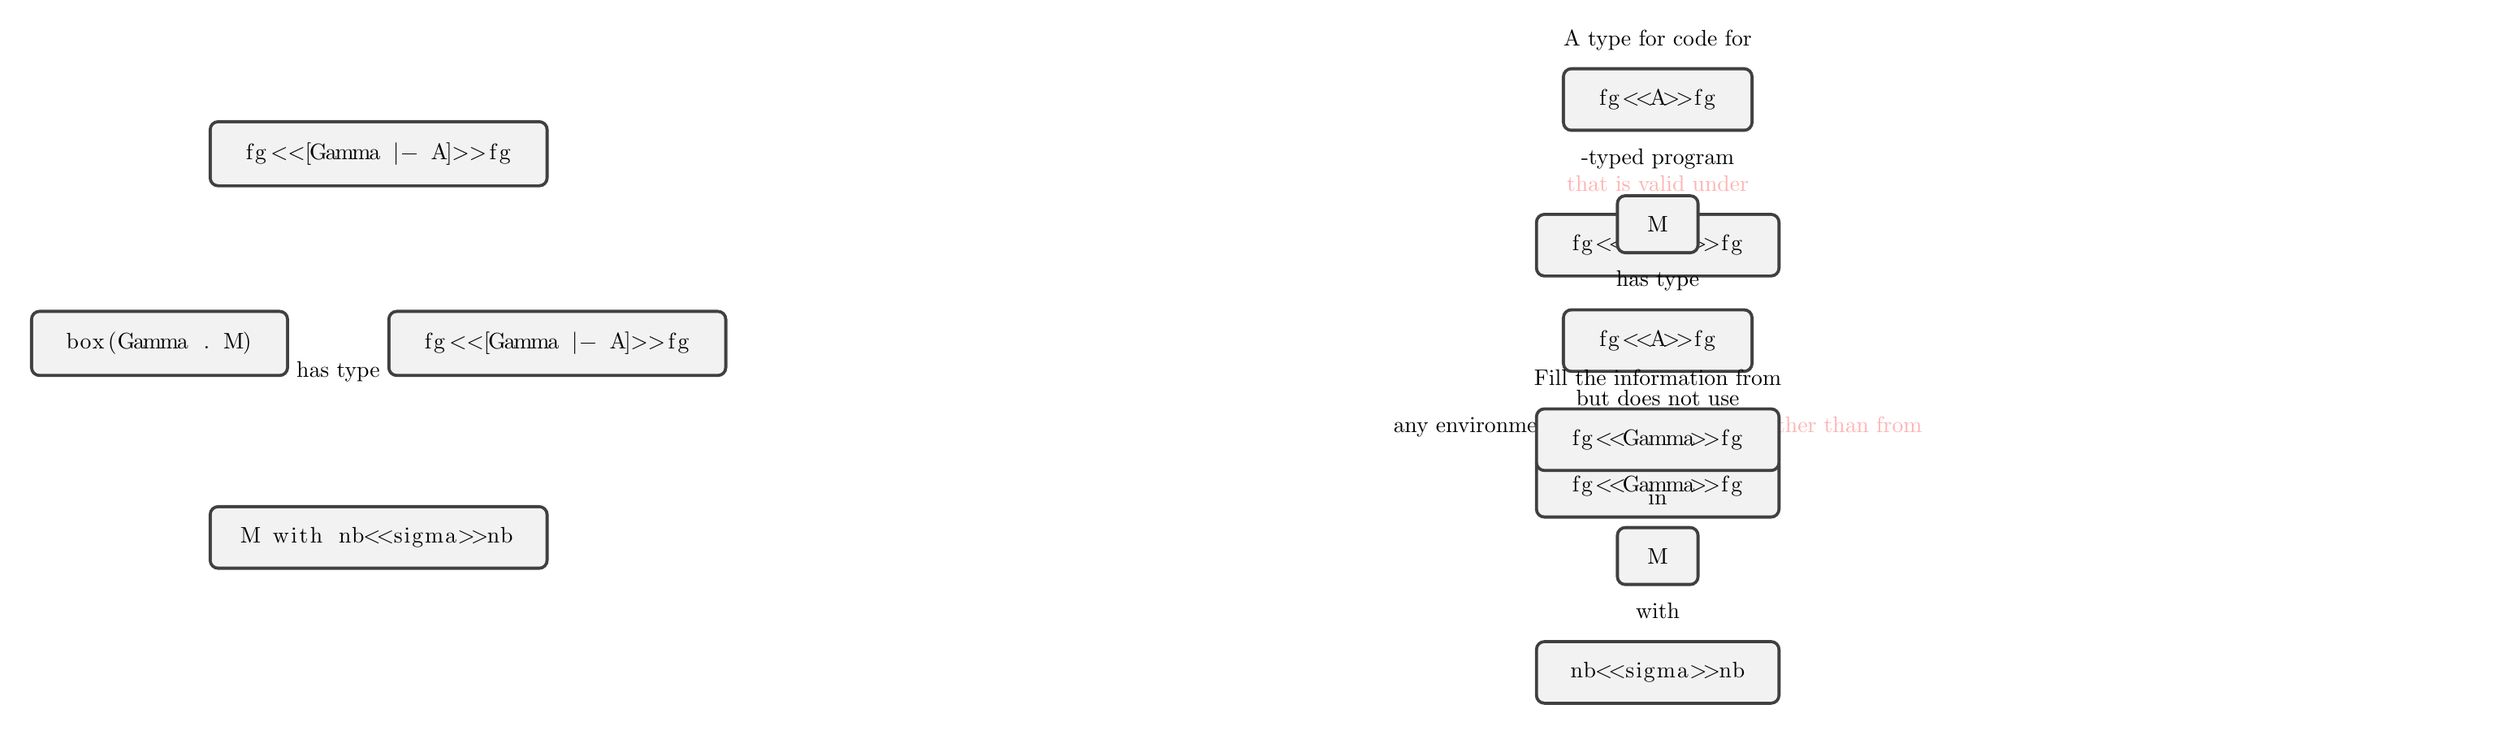
\begin{tikzpicture}
        \draw (0,3) node {\moeb{fg<<[Gamma |- A]>>fg}} (20,3) node[text width=10in,align=center] {A type for code for \moeb{fg<<A>>fg}-typed program\\ \color{red!30!white}{that is valid under \moeb{fg<<Gamma>>fg}}};
        \draw (0,0) node {\moeb{box(Gamma . M)} has type \moeb{fg<<[Gamma |- A]>>fg}} (20,0) node[text width=10in,align=center] {\moeb{M} has type \moeb{fg<<A>>fg} but does not use\\ any environment-specific information \color{red!30!white}{other than from \moeb{fg<<Gamma>>fg}}};
        \draw (0,-3) node {\moeb{M with nb<<sigma>>nb}} (20,-3) node[text width=10in,align=center] {Fill the information from \moeb{fg<<Gamma>>fg} in \moeb{M} with \moeb{nb<<sigma>>nb}};
      \end{tikzpicture}
    \end{tikzfigure*}
    \begin{tikzfigure*}[Metaprogram generating an open code fragment for the \(n\)-th item access]
      \lstinputlisting{src/open-int-nth.moebius}
    \end{tikzfigure*}
  If we execute \moeb{ws<<openIntNth>>ws 2}, we get
    \begin{tikzfigure*}
      \lstinputlisting{src/open-int-nth-2-result.moebius}
    \end{tikzfigure*}}

  \block{Levels: Necessity beyond Necessity}{
    \begin{tikzfigure*}
      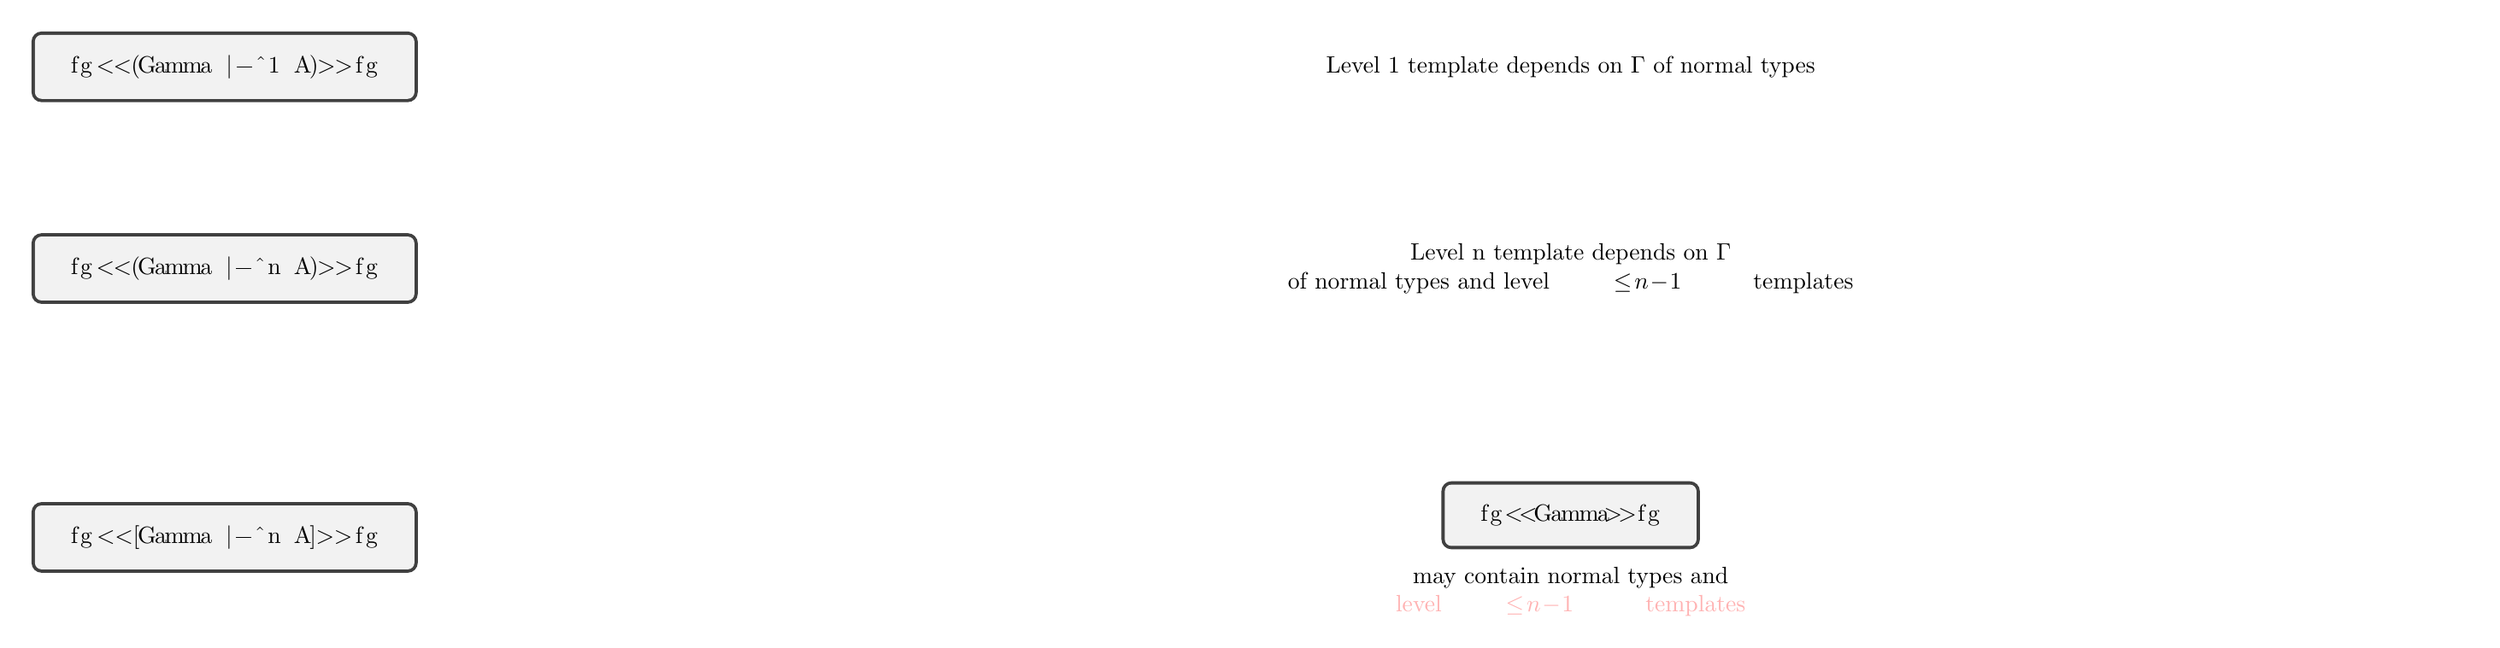
\begin{tikzpicture}
        \draw (0,3) node {\moeb{fg<<(Gamma |-^1 A)>>fg}} (20,3) node[text width=10.5in,align=center] {Level 1 template depends on \(\Gamma\) of normal types};
        \draw (0,0) node {\moeb{fg<<(Gamma |-^n A)>>fg}} (20,0) node[text width=10.5in,align=center] {Level n template depends on \(\Gamma\)\\ of normal types and level \makebox[1.1in]{\(\!\!\le{}\!n\!-\!1\)} templates};
        \draw (0,-4) node {\moeb{fg<<[Gamma |-^n A]>>fg}} (20,-4) node[text width=10.5in,align=center] {\moeb{fg<<Gamma>>fg} may contain normal types and\\ \color{red!30!white}{level \makebox[1.1in]{\(\!\!\le{}\!n\!-\!1\)} templates}};
      \end{tikzpicture}
    \end{tikzfigure*}
    \begin{tikzfigure*}[Polymorphic metaprogram to get the \(n\)-th item in a list]
      \lstinputlisting{src/polymorphic-nth.moebius}
    \end{tikzfigure*}
    \begin{tikzfigure*}[Ill-typed metaprogram to get the \(n\)-th item in a list]
      \lstinputlisting{src/contextual-matching.moebius}
    \end{tikzfigure*}
  where the type of \moeb{u<<X>>u} is \moeb{(xs : 'a list |-^2 'a list)}}

  \block{References}{Pfenning\&Davies/Contextual Type/Moebius}
\end{columns}
\end{document}
